\documentclass[12pt, a4paper]{article}
\usepackage{amsmath}
\usepackage{graphicx, float, booktabs}
\usepackage[UTF8]{inputenc}
\usepackage{fancyhdr, pdfpages, lastpage}
\usepackage[coverpage,
%online,
forcolorpaper, pointsonright, nototals, noparttotals,
nosolutions,%
%answerkey,%
useforms]{eqexam}

\title[]{Final Exam}
\author{mscbf\textunderscore\ rm01\textunderscore\ tsa}
\subject[Module 9.3]{Time Series Analysis}
\date{Fall term}
%\keywords{Test~1, Section 001}
%\numVersions{3}
%\forVersion{a}
\university
{%
      Lucerne University of Applied Sciences
}
\email{simon.broda@hslu.ch}

\hfuzz = .7pt
\examNameLabel{Last name:}

\setlength{\headheight}{15pt}
\setlength{\footskip}{12pt}
\lheadeqe{}
\rheadeqe{}
\cheadeqe{}
\examSIDLabel{Given name:}
\begin{document}
\fancyhf{}
\lfoot{\tiny © Lucerne School of Business. Any redistribution or reproduction of part or all of the contents in any form is prohibited.}
\rfoot{Page \thepage/\pageref{LastPage}}
\lhead{MSCBF\textunderscore RM01\textunderscore TSA}
\chead{Course 9.3: Research Methods III}
\rhead{MOCK EXAM}
\pagestyle{fancy}
\maketitle
\newcounter{question}


\begin{exam}{Question 0}

\begin{instructions}[Question 0]
\end{instructions}
\begin{problem}[0]
Hi
\end{problem}
\end{exam}
\newpage
\stepcounter{question}
\begin{exam}{Question \thequestion}
\begin{instructions}[Question \thequestion]

\end{instructions}
\begin{problem}[6]
I have simulated 1000 observations $\{y_t\}$ from an ARMA($p$, $q$) model. Figure \ref{fig:corr} on Page \pageref{fig:corr} shows a plot of the correlogram. Based on it, what do you think $p$ and $q$ are, and why?
\begin{solution}[10cm]
The PACF becomes insignificant after 2 lags, whereas the ACF decays exponentially. This is indicative of an AR(2) process.
\end{solution}
\end{problem}
\begin{problem}[6]
The 11th sample autocorrelation (not shown in the graph) is $\hat{\tau}_{11} =-0.045$. Test if $\hat{\tau}_{11}$ is significantly different from zero.
\begin{solution}[10cm]

\begin{itemize}
\item The hypotheses are $H_0: \tau_{11} = 0$ vs.\ $H_a: \tau_{11}\neq 0$.
\item The test statistic is $\hat{\tau}_{11}$.
\item Its distribution is $\mathrm{N}(0, 1/T)$ under $H_0$.
\item The critical value is thus $1.96/\sqrt{1000} = 0.062$.
\item The observed test statistic is $\hat{\tau}_{11} =-0.045$.
\item Since $|-0.045| < 0.062$, we do not reject $H_0$.
\item Conclusion: $\tau_{11}$ is not significantly different from zero.
\end{itemize}
\end{solution}


\end{problem}
\begin{problem}[6]
The output in Figure \ref{fig:adf} on Page \pageref{fig:adf} shows the results of regressing $\Delta y_t$ (\texttt{y}) on $y_{t-1}$ (\texttt{x1}) and $\Delta y_{t-1}$ (\texttt{x2}). Use it to test if the data are integrated.
\begin{solution}[10cm]

\begin{itemize}
\item The hypotheses are $H_0: y_t$ is integrated of order 1 vs.\ $H_a: y_t$ is stationary.
\item The test statistic is the estimated coefficient on the lagged level, $y_{t-1}$ (\texttt{x1}).
\item Its follows a Dickey-Fuller distribution  under $H_0$.
\item The critical value is -2.86, because a constant has been included.
\item The observed test statistic is -6.52.
\item Since $-6.52 < -2.86$, we reject $H_0$.
\item Conclusion: the data are stationary.
\end{itemize}
\end{solution}
\end{problem}
\begin{problem}[3]
I have estimated a particular ARMA model. The estimation output is shown in Figure \ref{fig:ar2} on Page \pageref{fig:ar2}. Write down the estimated model in equation form.
\begin{solution}[10cm]
The estimated AR(2) model is
\[
y_t =0.2158\cdot (1-0.5236-0.3595) +  0.5236\cdot  y_{t-1} + 0.3595 \cdot y_{t-2}.
\]
Note \texttt{archmodel}'s peculiar interpretation of the intercept, \texttt{const}: in our notation, it corresponds to $\hat{\alpha}/ (1-\hat{\phi}_1-\hat{\phi}_2)$, so that $\hat{\alpha} = \mathtt{const}\cdot (1-\hat{\phi}_1 - \hat{\phi_2})$. See the exercises.
\end{solution}
\end{problem}
\begin{problem}[6]
Use the estimated model from the previous question to forecast the value of the series at $t=1001$. You may need some of the values below.
\begin{center}
\begin{tabular}{lrr}
\toprule
$t$ & $y_t$ & $u_t$\\
\midrule
999 & -0.77 & -4.18\\
1000& -0.75 & -1.41\\
\bottomrule
\end{tabular}
\end{center}
\begin{solution}[5cm]
The forecast is
\begin{align*}
\widehat{y}_{1001} &= \mathtt{const}\cdot (1-\hat{\phi}_1 - \hat{\phi_2})+\hat{\phi}_1\cdot  y_{1000} + \hat{\phi}_2 \cdot y_{999}\\
&=  0.2158 \cdot (1-0.5236-0.3595) + 0.5236\cdot  (-0.75) + 0.3595 \cdot (-0.77)\\
&= -0.644.
\end{align*}
\end{solution}
\end{problem}

\end{exam}


\newpage
\stepcounter{question}
\begin{exam}{Question \thequestion}
\begin{instructions}[Question \thequestion]
In this exercise, we analyze the daily returns on Tesla stock between 6/29/2010 and 12/14/2022. The returns are shown in Figure \ref{fig:returns}.
\begin{figure}[H]
\begin{center}
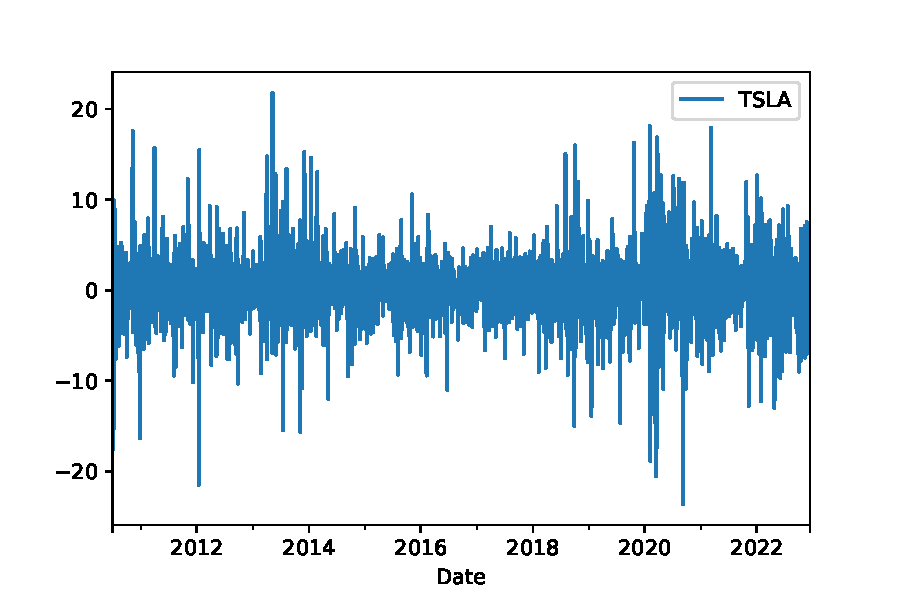
\includegraphics[width=0.5\textwidth]{tsla}
\end{center}
\caption{Returns on Tesla stock}\label{fig:returns}
\end{figure}
The data clearly display volatility clustering, which we want to model using a GARCH model. The output is shown in Figure \ref{fig:garch} on Page \pageref{fig:garch}.
\end{instructions}
\begin{problem}[3]
Write the model down as an equation (only the volatility equation).
\begin{solution}[4cm]
\[
\sigma^2_{t+1} = 0.14 + 0.0323 \cdot  u_t^2 + 0.9564 \cdot \sigma_t^2.
\]
\end{solution}
\end{problem}
\begin{problem}[6]
Does your model incorporate a leverage effect? Justify your answer.
\begin{solution}[7cm]
No. Since $u_t$ (the demeaned return) only enters as its square, the news impact curve is symmetric: volatility reacts equally strongly to a positive and negative shock of the same magnitude.
\end{solution}
\end{problem}
\begin{problem}[6]
Explain what the standardized residuals from a GARCH model are, ideally with an equation. Also, explain what their properties should be if the volatility model is correct.
\begin{solution}[10cm]
The standardized residuals are defined as $\hat{z}_t=\frac{r_t-\hat{\mu}_t}{\hat{\sigma}_t}$. If the model for $\sigma_t$ is correct, then they should no longer display volatility clustering. This means that there should be no autocorrelation in their squares.
\end{solution}
\end{problem}
\begin{problem}[6]
Regressing the squared standardized residuals on an intercept and 5 of their own lags results in an $R^2$ of 0.00364. Use this to test if the GARCH model has successfully removed the volatility clustering.
\begin{solution}[10cm]
This is an ARCH-LM test.
\begin{itemize}
\item The hypotheses are $H_0:$ no remaining volatility clustering vs.\ $H_a:$ there is remaining volatility clustering.
\item The test statistic is $T \cdot R^2$ in the auxiliary regression.
\item Its distribution is $\chi^2(5)$ under $H_0$.
\item The critical value is thus 11.07.
\item The observed test statistic is $3138 \cdot 0.00364 = 11.42$.
\item Since $11.42 > 11.07$, we reject $H_0$ (although barely).
\item Conclusion: Some volatility clustering remains.
\end{itemize}
\end{solution}
\end{problem}
\begin{problem}[6]
Use the model to predict the variance $\sigma^2_{t+1}$ for 12/15/2022, using the following values on 12/14/2022: $\hat{u}_t=-2.72$ and $\sigma^2_t = 15.198$.
\begin{solution}[10cm]
\begin{align*}
\widehat{\sigma}^2_{t+1} & = 0.14 + 0.0323 \cdot  u_t^2 + 0.9564 \cdot \sigma_t^2\\
& = 0.14 + 0.0323 \cdot (-2.72) ^2  + 0.9564 \cdot 15.198\\
& = 14.91.
\end{align*}

\end{solution}
\end{problem}
\end{exam}
\newpage
\stepcounter{question}
\begin{exam}{Question \thequestion}
\begin{instructions}[Question \thequestion]
We now turn our attention to Value at Risk forecasting.
\end{instructions}
\begin{problem}[6]
Use the model from the previous question to predict the 1\% Value at Risk for 12/15/2022. Note: If you weren't successful in predicting the variance in the previous question, you can use the value $\widehat{\sigma}^2_{t+1}=15.00$.
\begin{solution}[8cm]
The VaR forecast is
\begin{align*}
VaR^{0.01}_{t+1} &= -\mu_{t+1} - \sigma_{t+1} \cdot{} \Phi_{0.01}^{-1}\\
&= -\mu_{t+1} - \sigma_{t+1} \cdot \Phi_{0.01}^{-1}\\
&=-0.1118- \sqrt{14.91}\cdot(-2.326)\\
&=8.87.
\end{align*}
\end{solution}
\end{problem}
\begin{problem*}[\auto]
In a backtesting exercise, we have created 1\% VaR forecasts for the entire sample. From this and the returns, we have created the hit series $\{I_t\}$.
\begin{parts}
\item\PTs{6} Explain how the hit series is defined, and how many times you expect it to equal 1 if the VaR model is correct.
\begin{solution}[10cm]
The hit series equals 1 whenever a VaR violation occurs, i.e.,
\begin{equation*}
I_{t+1}=\left\{
\begin{array}{cc}
1, & \text{if }R_{t+1}<-VaR_{t+1}^{p}, \\
0, & \text{if }R_{t+1}>-VaR_{t+1}^{p}.%
\end{array}%
\right.
\end{equation*}
If the model is correct, we would expect a violation 1\% of the time. Since $T=3138$, we would therefore expect around 31 VaR violations.
\end{solution}

\item\PTs{6}  Figure \ref{fig:var} on page \pageref{fig:var} shows the result of regressing $(I_t-0.01)$ on an intercept and $I_{t-1}$. Use it to test the independence of the VaR violations.
\begin{solution}[10cm]
\begin{itemize}
\item The hypotheses are $H_0:$ the VaR violations are independent vs.\ $H_a:$ they are not.
\item The test statistic is the $t$ statistic for the lagged hit series.
\item Its distribution is (asymptotically) standard normal under $H_0$.
\item The critical value is thus 1.96.
\item The observed test statistic is $1.187$.
\item Since $|1.187| < 1.96$, we do not reject $H_0$.
\item Conclusion: there is no evidence of dependence between the VaR violations.
\end{itemize}
Note: in this case, since I didn't delete the $p$-value, you could alternatively have answered as follows.
\begin{itemize}
\item The hypotheses are $H_0:$ the VaR violations are independent vs.\ $H_a:$ they are not.
\item The test statistic is the $t$ statistic for the lagged hit series.
\item The observed $p$-value is $0.235>0.05$, so we do not reject $H_0$.
\item Conclusion: there is no evidence of dependence between the VaR violations.
\end{itemize}
\end{solution}
%\item\PTs{6}  Using the same output,
%\begin{solution}[10cm]
%\end{solution}

\end{parts}
\end{problem*}
\end{exam}

\newpage
\stepcounter{question}
\begin{exam}{Question \thequestion}
\begin{instructions}[Question \thequestion]
Answer the questions below.
\end{instructions}

\begin{problem*}[\auto]
\begin{parts}
\item\PTs{3}
Spurious regressions can occur between cointegrated variables.
\bigskip
\begin{answers}{3} % specify tabular any with 6 columns
    \bChoices
        \Ans0 True  \eAns0
        \Ans1 False \eAns0
    \eChoices
    \end{answers}
\item\PTs{3}
In a stationary time series, shocks $U_t$ have a transitory effect on the future of the series.
\bigskip
\begin{answers}{3} % specify tabular any with 6 columns
    \bChoices
        \Ans1 True  \eAns0
        \Ans0 False \eAns0
    \eChoices
    \end{answers}
\item\PTs{3}
An ARCH($q$) model for the returns corresponds to an AR($q$) for the squared returns.
\bigskip
\begin{answers}{3} % specify tabular any with 6 columns
    \bChoices
        \Ans1 True  \eAns0
        \Ans0 False \eAns0
    \eChoices
    \end{answers}

\item\PTs{3}
The order $q$ of an MA($q$) model can be determined from the correlogram.
\bigskip
\begin{answers}{3} % specify tabular any with 6 columns
    \bChoices
        \Ans1 True  \eAns0
        \Ans0 False \eAns0
    \eChoices
    \end{answers}

\item\PTs{3}
In the presence of the leverage effect, the news impact curve is steeper to the right of the origin than to the left.
\bigskip
\begin{answers}{3} % specify tabular any with 6 columns
    \bChoices
        \Ans0 True  \eAns0
        \Ans1 False \eAns0
    \eChoices
    \end{answers}
\item\PTs{3}
A VaR model is correctly specified if no VaR violations occur.
\bigskip
\begin{answers}{3} % specify tabular any with 6 columns
    \bChoices
        \Ans0 True  \eAns
        \Ans1 False \eAns0
    \eChoices
    \end{answers}

\end{parts}
\end{problem*}
\end{exam}

\mbox{}
\vfill
\begin{center}
\huge\bfseries End of exam.
\end{center}
\vfill
\newpage
\begin{figure}[H]
\begin{center}
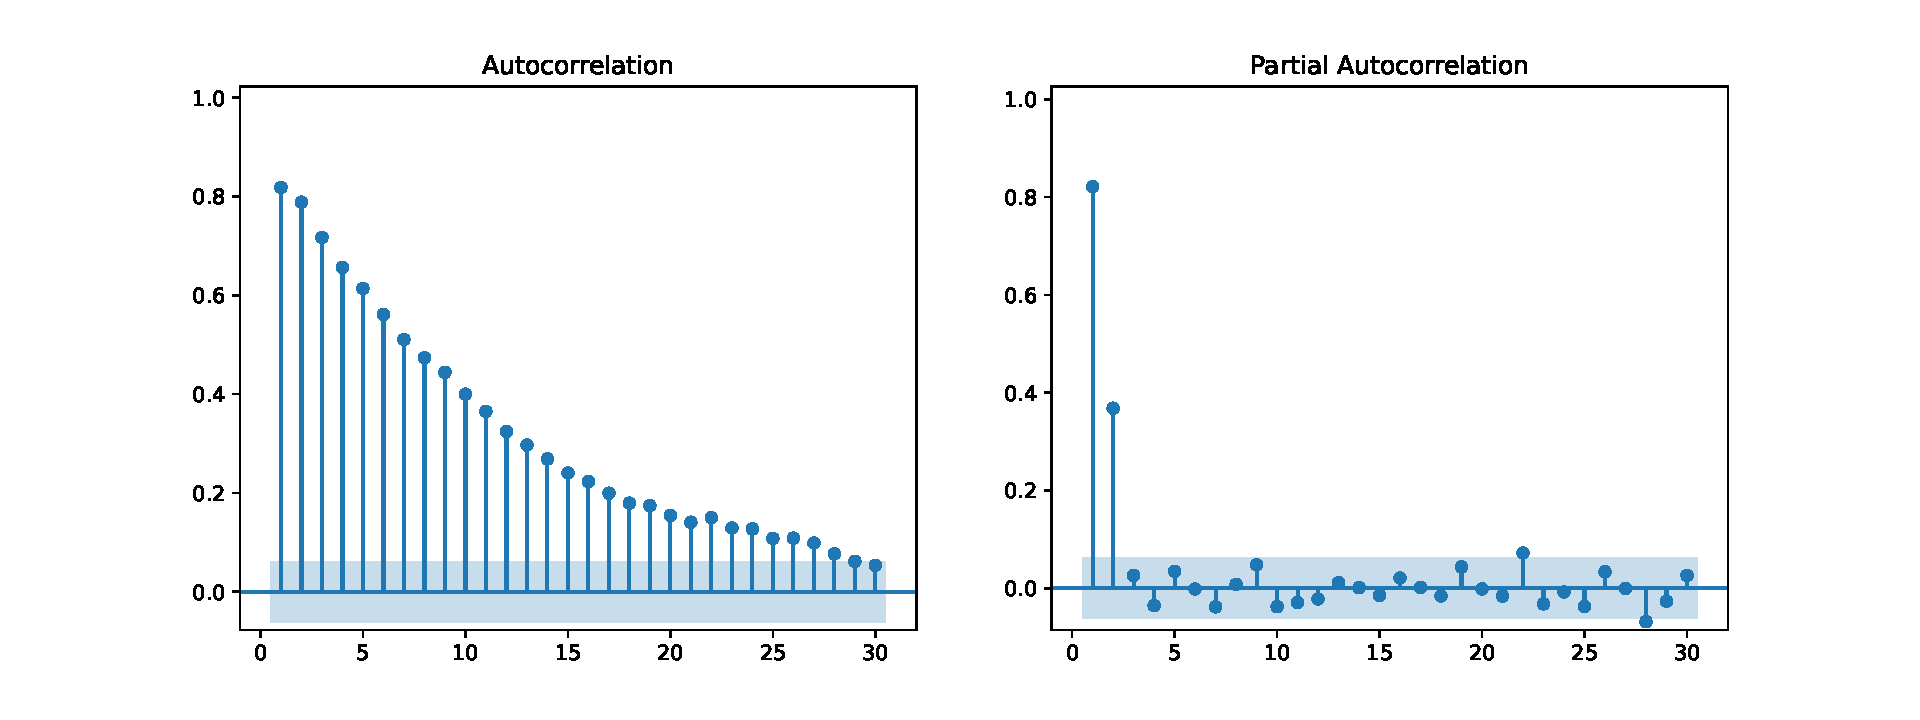
\includegraphics[width=\textwidth]{correlogram_ar2}
\end{center}
\caption{Correlogram of simulated data.}\label{fig:corr}
\end{figure}
\begin{figure}[H]
\footnotesize
\begin{verbatim}
                            OLS Regression Results
==============================================================================
Dep. Variable:                      y   R-squared:                       0.208
Model:                            OLS   Adj. R-squared:                  0.207
Method:                 Least Squares   F-statistic:                     130.9
Date:                Mon, 16 Oct 2023   Prob (F-statistic):           3.47e-51
Time:                        15:04:00   Log-Likelihood:                -2086.9
No. Observations:                 998   AIC:                             4180.
Df Residuals:                     995   BIC:                             4195.
Df Model:                           2
Covariance Type:            nonrobust
==============================================================================
                 coef    std err          t      P>|t|      [0.025      0.975]
------------------------------------------------------------------------------
x1            -0.1161      0.018     -6.520      0.000      -0.151      -0.081
x2            -0.3594      0.030    -12.164      0.000      -0.417      -0.301
const          0.0309      0.062      0.497      0.619      -0.091       0.153
==============================================================================
Omnibus:                        0.529   Durbin-Watson:                   2.023
Prob(Omnibus):                  0.768   Jarque-Bera (JB):                0.404
Skew:                           0.003   Prob(JB):                        0.817
Kurtosis:                       3.098   Cond. No.                         3.76
==============================================================================

\end{verbatim}
\caption{Output for ADF test.}\label{fig:adf}
\end{figure}
\begin{figure}[H]
\footnotesize
\begin{verbatim}
                               SARIMAX Results
==============================================================================
Dep. Variable:                      y   No. Observations:                 1000
Model:                 ARIMA(2, 0, 0)   Log Likelihood               -2091.958
Date:                Mon, 16 Oct 2023   AIC                           4191.917
Time:                        15:10:43   BIC                           4211.548
Sample:                             0   HQIC                          4199.378
                               - 1000
Covariance Type:                  opg
==============================================================================
                 coef    std err          z      P>|z|      [0.025      0.975]
------------------------------------------------------------------------------
const          0.2158      0.528      0.409      0.683      -0.818       1.250
ar.L1          0.5236      0.032     16.396      0.000       0.461       0.586
ar.L2          0.3595      0.032     11.326      0.000       0.297       0.422
sigma2         3.8369      0.169     22.770      0.000       3.507       4.167
===================================================================================
Ljung-Box (L1) (Q):                   0.13   Jarque-Bera (JB):                 0.36
Prob(Q):                              0.71   Prob(JB):                         0.83
Heteroskedasticity (H):               0.86   Skew:                             0.00
Prob(H) (two-sided):                  0.18   Kurtosis:                         3.09
===================================================================================
\end{verbatim}
\caption{Estimated ARMA model.}\label{fig:ar2}
\end{figure}

\begin{figure}[H]
\footnotesize
\begin{verbatim}
                     Constant Mean - GARCH Model Results
==============================================================================
Dep. Variable:                   TSLA   R-squared:                       0.000
Mean Model:             Constant Mean   Adj. R-squared:                  0.000
Vol Model:                      GARCH   Log-Likelihood:               -8267.70
Distribution:                  Normal   AIC:                           16543.4
Method:            Maximum Likelihood   BIC:                           16567.6
                                        No. Observations:                 3138
Date:                Mon, Oct 16 2023   Df Residuals:                     3137
Time:                        15:33:03   Df Model:                            1
                                 Mean Model
===========================================================================
                 coef    std err          t      P>|t|     95.0% Conf. Int.
---------------------------------------------------------------------------
mu             0.1118  5.774e-02      1.936  5.281e-02 [-1.359e-03,  0.225]
                              Volatility Model
============================================================================
                 coef    std err          t      P>|t|      95.0% Conf. Int.
----------------------------------------------------------------------------
omega          0.1400      0.117      1.196      0.232  [-8.938e-02,  0.369]
alpha[1]       0.0323  1.341e-02      2.409  1.599e-02 [6.024e-03,5.859e-02]
beta[1]        0.9564  2.205e-02     43.369      0.000     [  0.913,  1.000]
============================================================================
\end{verbatim}
\caption{Estimated GARCH model.}\label{fig:garch}
\end{figure}
\begin{figure}[H]
\footnotesize
\begin{verbatim}
                             OLS Regression Results
================================================================================
Dep. Variable:     np.subtract(I, 0.01)   R-squared:                       0.000
Model:                              OLS   Adj. R-squared:                  0.000
Method:                   Least Squares   F-statistic:                     1.409
Date:                  Mon, 16 Oct 2023   Prob (F-statistic):              0.235
Time:                          18:54:56   Log-Likelihood:                 1976.8
No. Observations:                  3137   AIC:                            -3950.
Df Residuals:                      3135   BIC:                            -3938.
Df Model:                             1
Covariance Type:              nonrobust
==============================================================================
                 coef    std err          t      P>|t|      [0.025      0.975]
------------------------------------------------------------------------------
b0             0.0065      0.002      2.817      0.005       0.002       0.011
I.shift(1)     0.0212      0.018      1.187      0.235      -0.014       0.056
==============================================================================
Omnibus:                     4069.691   Durbin-Watson:                   2.001
Prob(Omnibus):                  0.000   Jarque-Bera (JB):           412759.104
Skew:                           7.492   Prob(JB):                         0.00
Kurtosis:                      57.160   Cond. No.                         7.76
==============================================================================
\end{verbatim}
\caption{Test regression for the Value at Risk backtest.}\label{fig:var}
\end{figure}


\end{document}
